\documentclass[class=article, crop=false]{standalone}
\usepackage{my_preamble}
\begin{document}
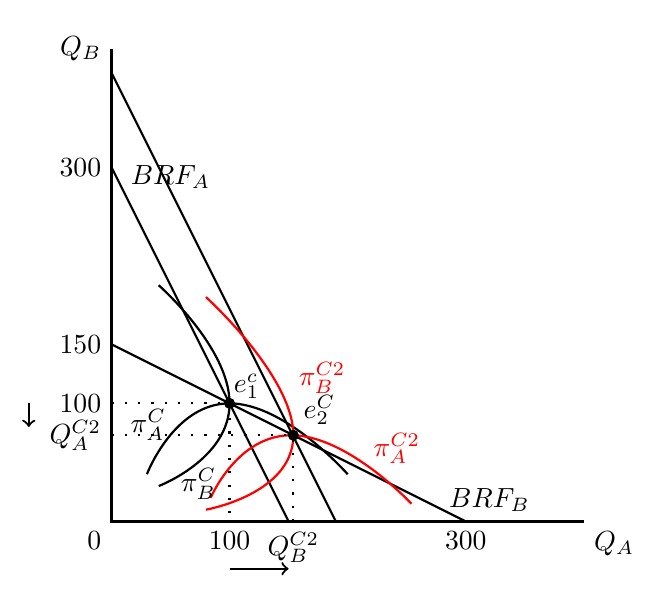
\begin{tikzpicture}[thick,font=\sffamily,scale=1.5]
	%axis
	 \draw (0,4) node[left]{$Q_{B}$} -- (0,0) node[below left] {$0$} -- (4,0) node[below right]{$Q_{A}$};
	  
	 %BRFs
	\draw[] (0,3) -- (1.5,0); %BRF A
	\draw[] (0,3.8) -- (1.9,0); %BRF A 2
	\draw[] (0,1.5) -- (3,0); %BRF B

	%Iso-profits
	\draw[] plot [smooth, tension=1] coordinates {(0.3,0.4) (1,1) (2,0.4)}; %A's iso-profit 1
	\draw[red] plot [smooth, tension=1] coordinates {(0.84,0.2) (1.54,0.73) (2.54,0.15)}; %A's iso-profit 2
	\draw[] plot [smooth, tension=1] coordinates {(0.4,0.3) (1,1) (0.4,2)}; %B's iso-profit 1
	\draw[red] plot [smooth, tension=1] coordinates {(0.8,0.1) (1.54,0.73) (0.8,1.9)}; %B's iso-profit 2
	
	%labels
	\node[below] at (0.5,3.1) {$BRF_{A}$}; %BRF A label
	\node[above] at (3.2,0) {$BRF_{B}$}; %BRF B label
	%\node[below] at (1.5,0) {$150$}; %A's monopoly quantity
	\node[left] at (0,1.5) {$150$}; %B's monopoly quantity
	\node[below] at (3,0) {$300$}; %A's PC quantity
	\node[left] at (0,3) {$300$}; %B's PC quantity
	\node[above left]at (0.55,0.6) {$\pi_A^C$}; %A's iso-profit 1 label
	\node[above right]at (0.5,0.1) {$\pi_B^C$}; %B's iso-profit 1 label
	\node[above left, red]at (2.7,0.4) {$\pi_A^{C2}$}; %A's iso-profit 2 label
	\node[above right, red]at (1.5,1) {$\pi_B^{C2}$}; %B's iso-profit 2 label
	
	
	%equilibria labels
	\node[style={fill=black,circle,inner sep=0pt,minimum size=4pt}] at (1,1) { };
	\node[above right]at (0.95,0.95) {$e^{c}_1$};
	\node[style={fill=black,circle,inner sep=0pt,minimum size=4pt}] at (1.54,0.73) { };
	\node[above right]at (1.54,0.73) {$e^{C}_2$};
	
	%dotted lines	
	\draw[loosely dotted] (0,1) node[left]{$100$} -| node[pos=0.25,below=3mm] {} (1,0) node[below]{$100$}; %cournot dotted lines
	\draw[loosely dotted] (0,0.73) node[left]{$Q^{C2}_A$} -| node[pos=0.25,below=3mm] {} (1.54,0) node[below]{$Q^{C2}_B$}; %new dotted lines
	
	%arrows
	\draw [->] (1,-0.4) -- (1.5,-0.4); %x arrow
	\draw [->] (-0.7,1) -- (-0.7,0.8); %y arrow
\end{tikzpicture}
\end{document}